\section{Results and analysis}
\begin{frame}<beamer>{Outline}
    \tableofcontents[currentsection,currentsubsection]
  \end{frame}
 \begin{frame}{Results}
     \begin{itemize}
         \item{ \textbf{Neural Networks 1 (Net-1h)}
         }
%         \item { Accuracy is 97.78\%} 
     \end{itemize}
     
		\begin{center}
		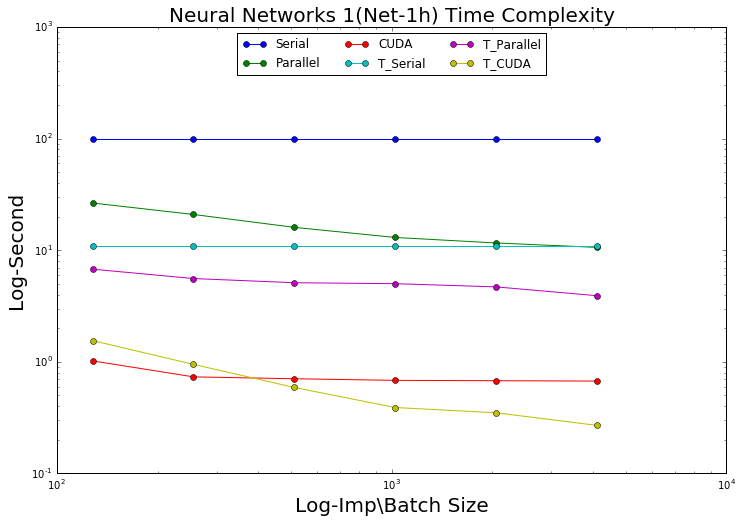
\includegraphics[width=3.4in]{nn1_time.png}
		\end{center}

 \end{frame}
 
\begin{frame}{Results (contd.)}
     \begin{itemize}
         \item{ \textbf{Neural Networks 2 (Net-2h)}
         }
%         \item { Accuracy is ???\%} 
     \end{itemize}
     
		\begin{center}
		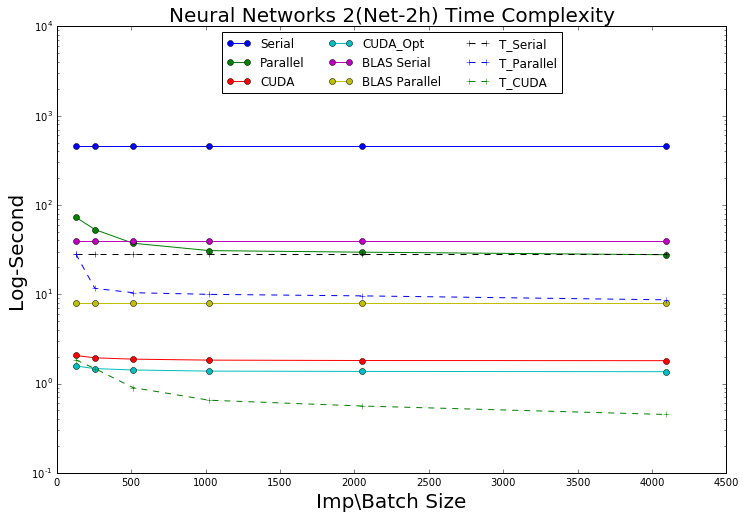
\includegraphics[width=3.4in]{nn2_time.png}
		\end{center}

 \end{frame} 

\begin{frame}{Results (contd.)}
     \begin{itemize}
         \item{ \textbf{Neural Networks 1 (Net-1h) - GFLOPS}
         }
     \end{itemize}
     
		\begin{center}
		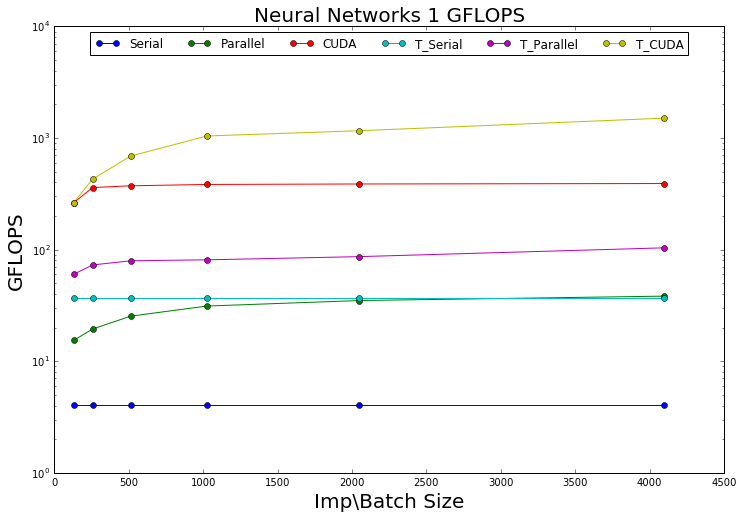
\includegraphics[width=3.4in]{nn1_gflops.png}
		\end{center}

 \end{frame} 

\begin{frame}{Results (contd.)}
     \begin{itemize}
         \item{ \textbf{Neural Networks 2 (Net-2h)- GFLOPS}
         }
     \end{itemize}
     
		\begin{center}
		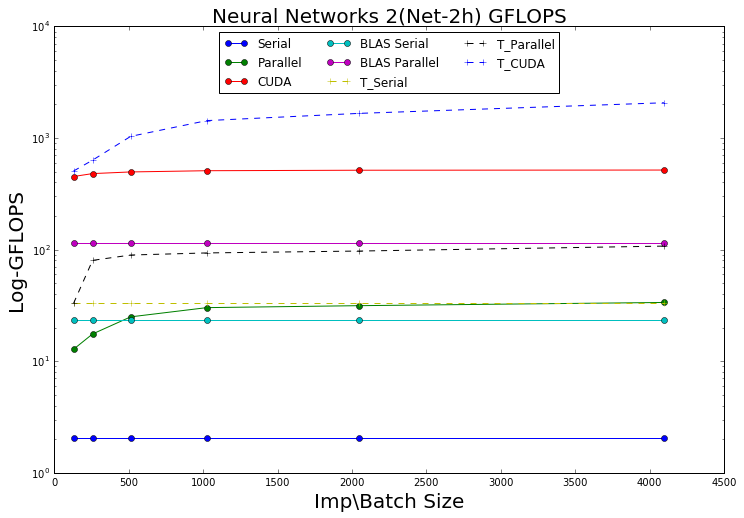
\includegraphics[width=3.4in]{nn2_gflops.png}
		\end{center}

 \end{frame} 

 
 \begin{frame}{Analysis}
 	\begin{itemize}
 	\item {Naive implementation}
 	\begin{itemize}
 	\item {Parallel computing provides faster training time than serial implementation.}
 	\item {By increasing the mini batch size, we can much faster training time.}
 	\end{itemize}
 	\item {\textbf{BLAS}}
 	\begin{itemize}
 	\item {Significantly improved results (even faster than Theano) with BLAS.}
 	\item {It is able to parallelize each Matrix-vector product.}
 	\item { This way shows that the optimized parallelism gives speed-up over Naive serial implementation.}
	\end{itemize}
	\item {\textbf{Bottlenecks}}
	\begin{itemize}
	\item {Shared memory bank conflicts reduce the parallelism.}
	\item {When the number of neurons between layers is not perfect multiple of 32 then some threads do not participate in the computation but just wait.}
	\item {As a result, it causes degraded parallelism.}
	\end{itemize}
 	\end{itemize}
 
 \end{frame}



